\section{Measure Theory and Integration}

Measure theory is a rich field in mathematics, which helps us later develop probability theory, as we will see that probability is just a measure of possibility. Therefore, in this section, we will discuss fundamental and sufficient concepts and theorems in this field. Measure theory was really motivated by measuring in normal senses. Specifically, the length of an interval $I=[a,b]$ in $\RR$ is measured by $\ell(I)=|b-a|$, the area of a rectangle $S = [a_1,b_1]\times [a_2,b_2] = I_1\times I_2$ in $\RR^2$ is $\ell(I_1)\cdot\ell(I_2)$. More generally, given intervals $I_k = [a_k,b_k], k = 1,\ldots, n$, the volume of the box $B= I_1\times \ldots \times I_n$ in  $\RR^d$ is $\prod\limits_{k=1}^d \ell(I_k)$. For a triangle, we calculate its area by cutting and reshaping it to a rectangle. For a circle, we divide it into multiple triangles and try to calculate the total area when the number of divisions tend to infinity, as illustrated in Figure \ref{figure:circle}. When encountering with more complex-shaped regions, as soon as it can be modeled as an equation or a system of equations in the coordinated plane, the usual Riemann integral approach is basically a division of the regions to infinitely many rectangles or triangles. As a consequence, this raises a crucial question whether all subsets of $\RR^d$ are measurable, in the sense of length, area and volume that we talked about. In following Proposition \ref{proposition-vitali-set}, we will prove that our intuitive length measure cannot be applied for all subsets of $\RR$ \cite{vitali1905sul}.

\begin{figure}[ht]
  \centering
  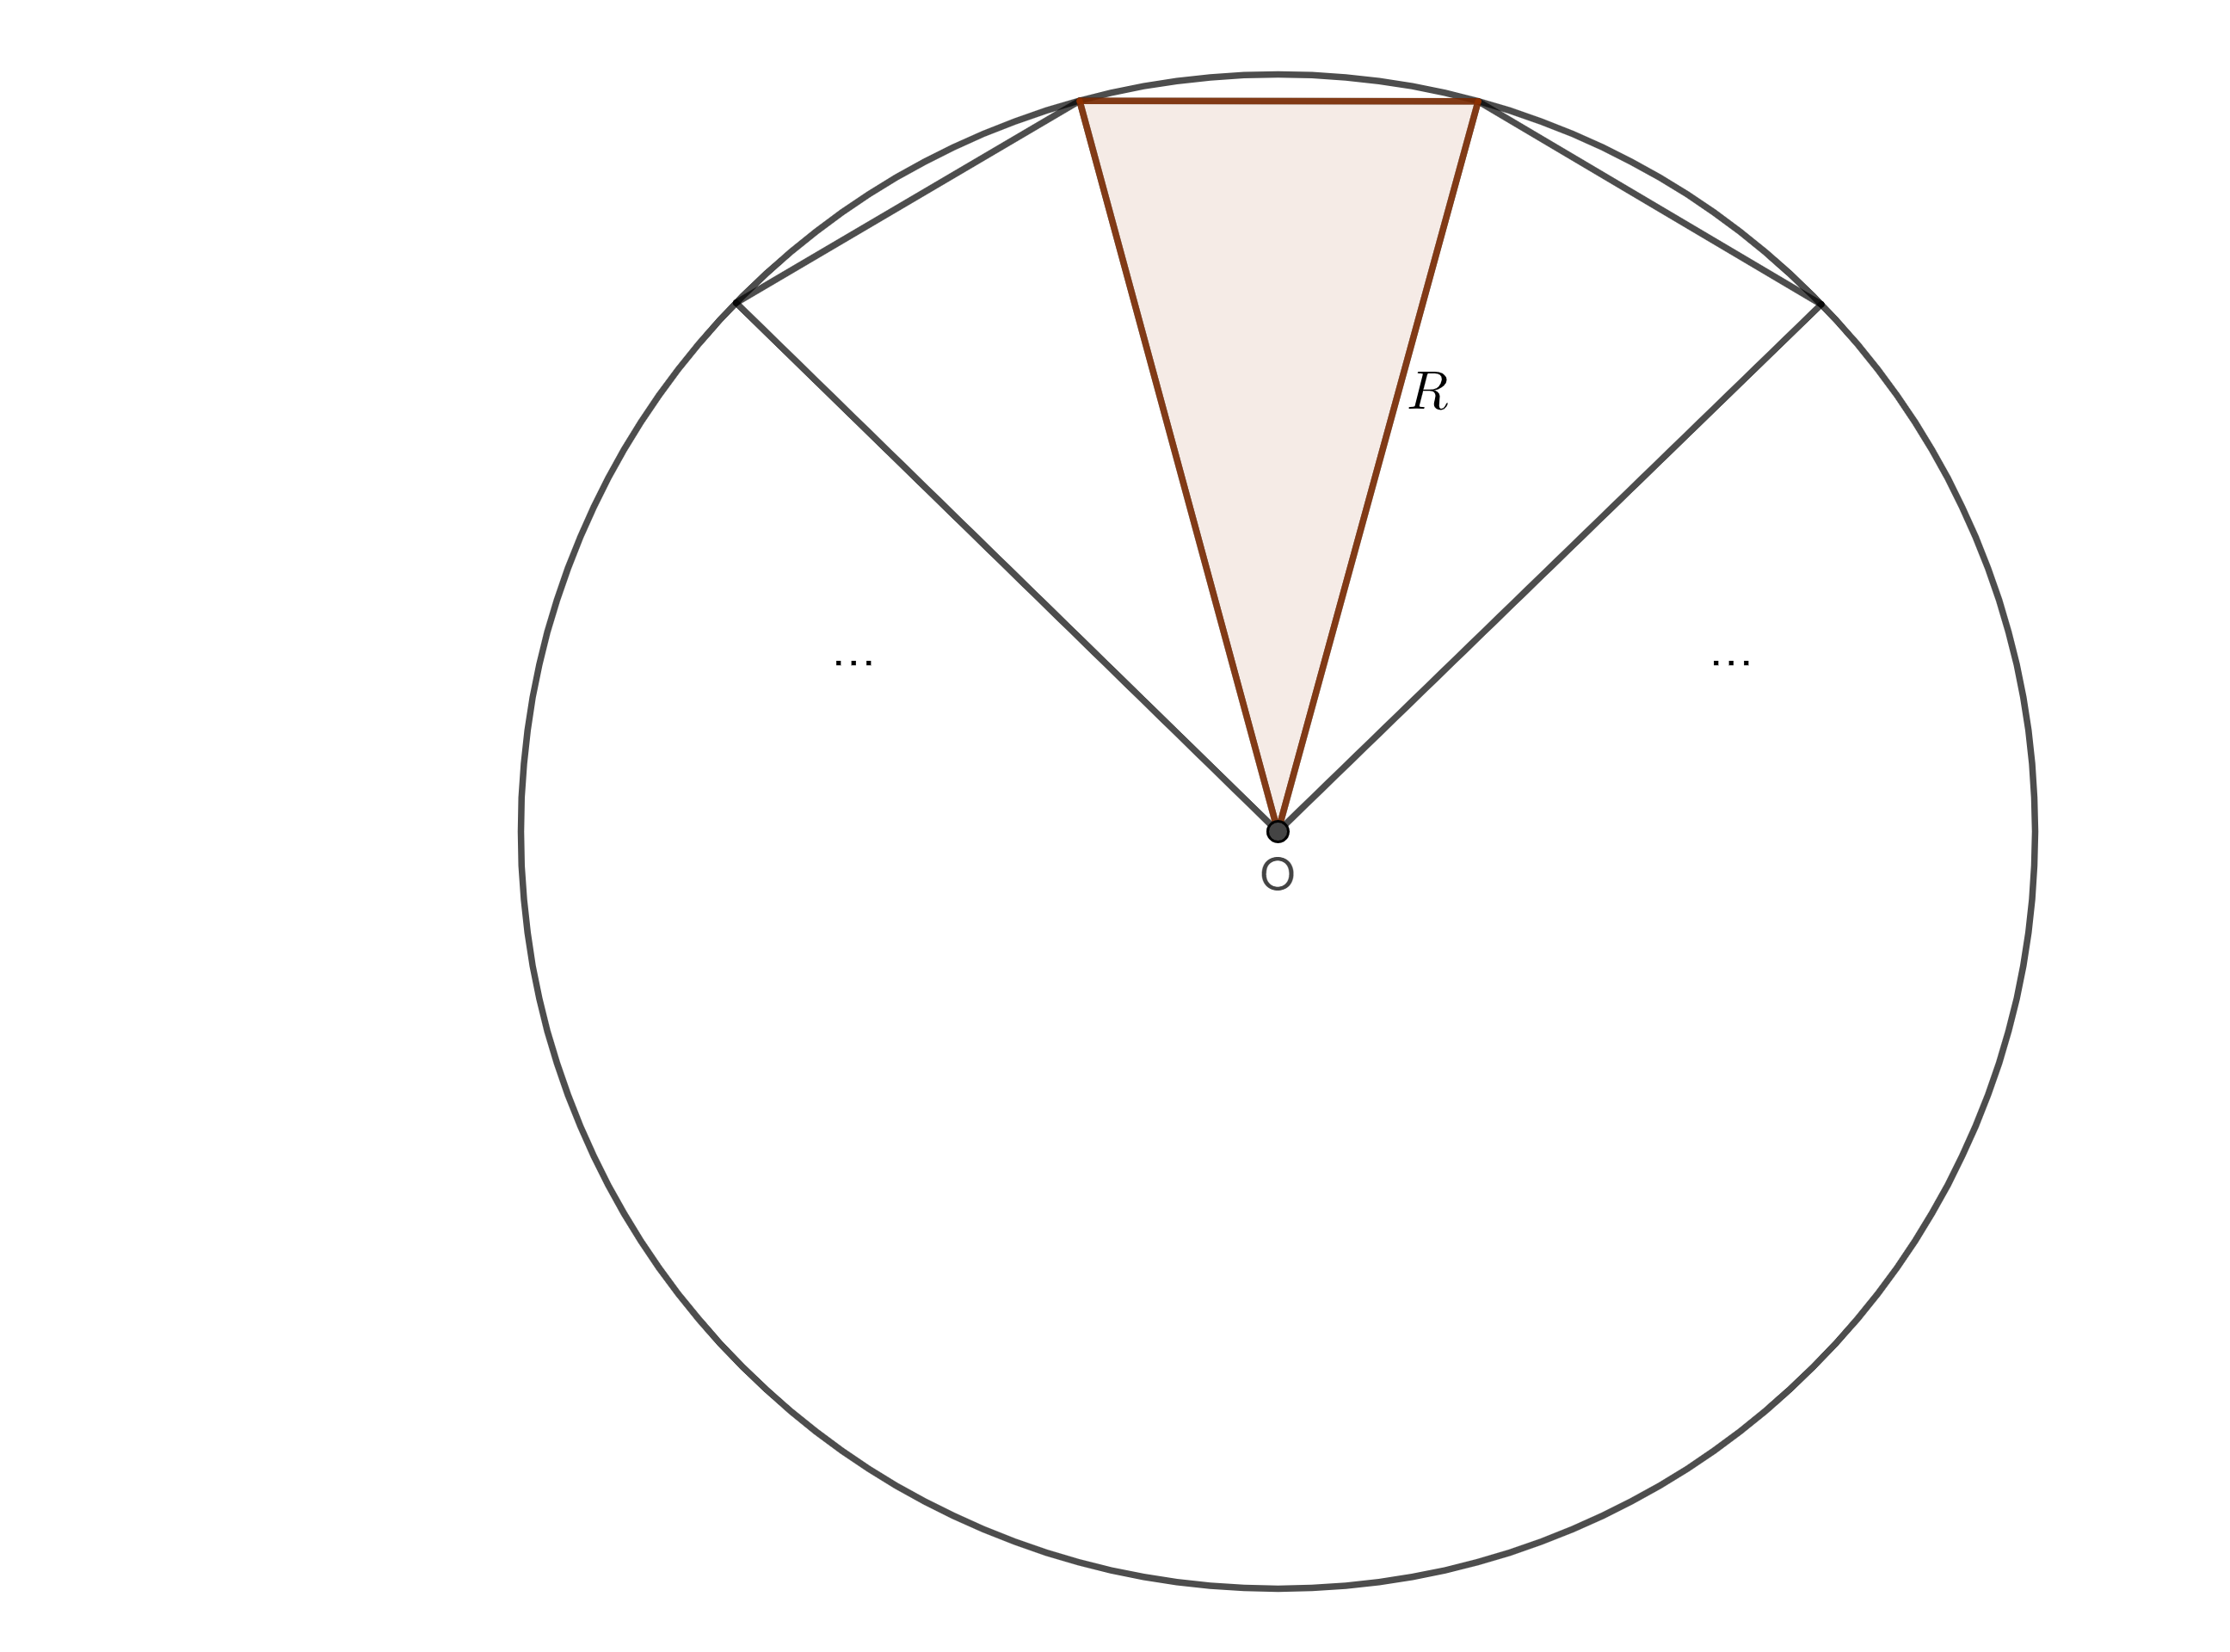
\includegraphics[width=0.4\linewidth]{img/circle.png}
  \vspace{0.5cm}
  \caption[Circle area approximation]{The area of a circle can be calculated by dividing it into equal isosceles triangles. As the number of triangles tends to infinity, the sum of bottom sides tends to the perimeter $2\pi R$ of the circle and the attitude of a triangle tends to $R$. Hence, the area is $A=\dfrac{1}{2}(2\pi R)R=\pi R^2$.}
  \label{figure:circle}
\end{figure}

\begin{proposition}[Vitali Set]
  \label{proposition-vitali-set}
  Suppose that there exists a function $\ell : \P(\RR) \to [0,\infty]$ from the power set of $\RR$ to the non-negative real numbers, such that
  \begin{enumerate}[label=(\arabic*)]
    \item $\ell(\varnothing) = 0$.
    \item $\ell([a,b]) = b-a$.
    \item If $E\subset F\subset \RR$, then $\ell(E)\le \ell(F)$.
    \item Translation invariance: for any $x\in\RR$, $\ell(E+x) = \ell(E)$.
    \item Countable additivity: if $E$ can be divided to a collection of disjoint intervals $\{I_k\}_{k\in \NN}$, then $\ell(E) = \sum\limits_{k=1}^\infty \ell(I_k).$
  \end{enumerate}
  Assuming the Axiom of Choice, we must have that $\ell(E) = 0, \forall E\in \P(\RR)$.
\end{proposition}

\begin{proof}
  By (2) and (3), we have $\ell((0,1])\le \ell([0,1]) = 1$. Let us define an equivalence relation \index{equivalence relation} on $(0,1]$ as
  $$x\sim y \Leftrightarrow x-y\in\QQ.$$
  Clearly, for any $x\in (0,1]$, we have the equivalence class
  $$[x] = \{y\in(0,1] : x-y\in \QQ\} = \{x+q: q\in \QQ, x+q\in (0,1]\}.$$

  Let $I$ be an index set for the equivalence classes. For each equivalence class, choose a representation $x_k, k \in I$ (we have made use of the Axiom of Choice here). Let $V=\{x_k\}_{k\in I}$. The set $V$ is called the Vitali set on $(0,1]$. Clearly, $V$ contains distinct elements. Let $(q_n)_{n\in\NN}$ be a sequence of $\QQ\cap(-1,1]$. Also, let $V_n = V + q_n$ for $n\in\NN$. We claim that the class $\{V_n\}_{n\in\NN}$ is distinct. Otherwise, suppose that there exist $m,n\in \NN$, where $m\ne n$ such that there exists $x\in V_n\cap V_m$. We have $x=y + q_n = z + q_m$, where $y,z\in A$ and $q_n,q_m\in\QQ$, implying that
  $$y-z = q_m-q_n\in \QQ.$$
  This means $y\sim z$, which contradicts to our construction of the equivalence classes.

  By (4) and (5), we have
  $$\ell((-1,2]) = \ell((-1,0]) + \ell((0,1]), \ell((1,2]) = 3\ell((0,1]).$$

  By (3), we have
  $$\ell(E_n) = \ell (A), \forall n\in\NN.$$

  Also, since $(0,1] \subset \bigcup\limits_{n=1}^\infty E_n \subset (-1,2]$, previous statements imply that
  $$\ell((0,1]) \le \ell\left(\bigcup\limits_{n=1}^\infty E_n\right) = \sum\limits_{k=1}^{\infty} \ell(A_k) = \sum_{k=1}^{\infty} \ell(A) \le 3\ell((0,1]).$$

  This implies $\ell(A)=0$, and also $\ell((0,1])=0$. Therefore,

  $$\ell(\RR) = \ell\left(\bigcup\limits_{m\in\ZZ}(m,m+1] \right) = \sum\limits_{m\in\ZZ} \ell((m,m+1])= \sum\limits_{m\in\ZZ} \ell((0,1]) = 0.$$

  Thus, $\ell$ coincides with the zero function. However, this measure of length is unavailing.
\end{proof}

After considering Proposition \ref{proposition-vitali-set}, we see that the concept of measure needs more diligent work than our normal measure calculation. This branch of real analysis establishes the general concept of measure and constructs different measures rather than length, area and volume. In this generalization, any abstract set $\Omega$ rather than $\RR^d$ are considered, along with the collection of measurable subsets of $\Omega$.

\subsection{Measure Space}

Let $\Omega$ be any abstract set, analogous to a region in $\RR^d$. In this subsection, we will define step-by-step what a collection of measurable subsets of $\Omega$ and which conditions a measure must meet. Consider the following real-life example. The collection of measurable subsets of $\Omega$ is called a $\sigma$-algebra.

\begin{definition}
  \label{definition:sigma-algebra}
  Given a set $\Omega$. A collection of subsets $\F$ of $\Omega$ is called a \textbf{$\sigma$-algebra}\index{$\sigma$-algebra} if
  \begin{enumerate}
    \item $\varnothing, \Omega\in\F$;
    \item If $A\in\F$, then $A^c\in\F$;
    \item If $A_1,A_2,\ldots\in\F$, then $A_1\cup A_2\cup\ldots\in\F$.
  \end{enumerate}
  The pair $(\Omega, \F)$ is called a \textbf{measurable space}\index{measurable space}.
\end{definition}

In Definition \ref{definition:sigma-algebra}, the first condition guarantees that the empty set and our whole initial set should be measurable. The second condition is interpreted as that if we can measure a subset, we should be able to measure the remaining. The third condition imitates our division approach when calculating complex-shaped regions in $\RR^d$. Before the definition of a measure, we consider some examples and derived technical theorems.

\begin{example}
  \label{example:1}
  Given a set $\Omega$, then $\{\varnothing, \Omega\}$ and the power set $2^\Omega$ are two trivial $\sigma$-algebras. Let $\Omega=\{1,2,3\}$, the collection $\F=\{\varnothing,\Omega, \{1\}, \{2,3\}\}$ is a $\sigma$-algebra on $\Omega$.
\end{example}

\begin{proposition}
  Let $\{\F_\alpha\}_{\alpha\in I}$ be an arbitrary family of $\sigma$-algebras on $\Omega$. Then the intersection $\F=\bigcap\limits_{\alpha\in I}\F_\alpha$ is a $\sigma$-algebra.
\end{proposition}

\begin{proof}
  We will check that $\F$ three conditions for a $\sigma$-algebra.

  Since $\varnothing,\Omega\in\F_\alpha,\forall\alpha\in I$, we have $\varnothing,\Omega\in\bigcap\limits_{\alpha\in I}\F_\alpha$.

  If $A\in\bigcap\limits_{\alpha\in I}\F_\alpha$, then $A\in \F_\alpha,\forall\alpha\in I$, leading to $A^c\in \F_\alpha,\forall\alpha\in I$. Hence, $A^c\in\bigcap\limits_{\alpha\in I}\F_\alpha.$

  Finally, if $A_i\in\F_\alpha,\forall i\in\ZZ^+,\forall \alpha\in I$, then $\bigcup\limits_{i\in\ZZ^+}A_i\in\F_\alpha,\forall\alpha\in I$. Therefore,
  $\bigcup\limits_{i\in\ZZ^+}A_i\in\bigcap\limits_{\alpha\in I}\F_\alpha.$
\end{proof}

\begin{remark}
  The union of $\sigma$-algebras on $\Omega$ is not necessarily a $\sigma$-algebra. For example,
  $$\F_1=\{\varnothing,\Omega, \{1\}, \{2,3\}\} \text{ and } \F_2=\{\varnothing,\Omega, \{2\}, \{1,3\}\}$$
  are two $\sigma$-algebras on $\Omega=\{1,2,3\}$, but
  $$\F=\F_1\cup\F_2=\{\varnothing,\Omega,\{1\},\{2\},\{2,3\},\{1,3\}\}$$ is not, since $\{3\}=\{2,3\}\cap\{1,3\}\notin \F$.
\end{remark}

Having mentioned in Example \ref{example:1}, any collection $\C$ of subsets of $\Omega$, has a trivial $\sigma$-algebra $2^\Omega$ that contains $\C$ i.e. $\C\subset2^\Omega$. Therefore, there exists the smallest $\sigma$-algebra containing $\C$.

\begin{theorem}
  \label{theorem:generated-sigma-algebra}
  Given a set $\Omega$ and a collection of its subsets $\C$, there exists the smallest $\sigma$-algebra containing $\C$, denoted by $\sigma(\C)$, given by
  $$\sigma(\C)=\bigcap\limits_{\alpha\in I}\F_\alpha,$$
  where $\{\F_\alpha\}_{\alpha\in I}$ is the set of $\sigma$-algebras containing $\C$. We also called $\sigma(\C)$ to be the $\sigma$-algebra generated by $\C$.
\end{theorem}

\begin{proof}
  Since $\sigma(\C)$ itself is a $\sigma$-algebra containing $\C$ so $\sigma(\C)\in\{\F_\alpha\}$, we have $\bigcap\limits_{\alpha\in I}\F_\alpha\subset \sigma(\C).$ In addition, $\bigcap\F_i$ is also a $\sigma$-algebra containing $\C$ and $\sigma(\C)$ is the smallest one, hence $\sigma(\C)\subset\bigcap\limits_{\alpha\in I}\F_i.$ Thus, $\sigma(\C)=\bigcap\limits_{\alpha\in I}\F_i$.
\end{proof}

\begin{example}
  Let $\Omega=\{1,2,3\}$. The collection $\C=\{\{1\}\}$ generates the $\sigma$-algebra $\F=\{\varnothing,\Omega,\{1\},\{2,3\}\}.$
\end{example}

\begin{definition}
  \label{definition-measure}
  Given a measurable space $(\Omega,\F)$, a function $\mu:\F\to\RR_+$ is called a \textbf{measure}\index{measure} if it satisfies
  \begin{enumerate}
    \item $\mu(\varnothing)=0$.
    \item Countable additivity: let $\{E_n\}_{n\in \NN}$ be a disjoint class of pairwise disjoint subsets of $\Omega$ in $\F$. Then
          \begin{equation}
            \mu\left(\bigcup\limits_{n=1}^\infty E_n\right)=\sum\limits_{i=n}^\infty \mu(E_n).
          \end{equation}
          The triplet $(\Omega,\F,\mu)$ is called a measure space.
  \end{enumerate}
\end{definition}

The conditions in Definition \ref{definition-measure} meet our intuition of what a measure should satisfy, namely the measure of the empty set is zero, the measure of any set is non-negative, and that the measure of a complex subset $A = \bigcup\limits_{n=1}^\infty E_n$ of $\Omega$ can be calculated by summing of the measures of distinct subsets $E_n$ for $n\in\NN$. The richness of measure theory is diligently developed from this fundamental concept of measure space.

% \begin{theorem}[Properties of a measure]
%   \begin{enumerate}
%     \item[]
%     \item Monotonicity\index{monotonicity}: if $A\subset B$, then $\mu(A)\le\mu(B)$.
%   \end{enumerate}
% \end{theorem}

\begin{example}
  \begin{enumerate}
    \item []
    \item Consider the measurable space $(\RR, \B(\RR))  $. The function of taking the length of open intervals on the real line
          $$\mu((x,y))=|y-x|,\forall x,y\in\RR,$$
          which an assumption that $\mu(\varnothing)=0$, is a measure. Three properties of a measure are satisfied trivially.
    \item Consider the measurable space $(\RR, \F)$, where $\F$ is any $\sigma$-algebra on $\RR$. Given $a\in\RR$. The indicator function $\mathbf{1}_a: \F\to\{0,1\}$ given by
          $$\begin{cases}
              \mathbf{1}_a(X)=1, & \text{ if } a\in X \\
              \mathbf{1}_a(X)=0, & \text{ otherwise }
            \end{cases}$$
          is a measure. We already have $\mathbf{1}_a(X)\ge0, \forall a\in X$. Let us check the other two properties of a measure for this function.
          \begin{itemize}
            \item Since $a\notin\varnothing$, we have $\mathbf{1}_a(\varnothing)=0$.
            \item For disjoints $X_1,X_2,\ldots$ it cannot be the case that there are two of them contain $a$. If $a\notin X_k,\forall k\in\ZZ^+$, then countable additivity holds since both sides are zero. Otherwise, if there exists $k\in \ZZ^+$ such that $a\in X_k$, then it follows that $$a\notin X_\ell, \forall \ell\ne k,$$ implying both sides are one.
          \end{itemize}
  \end{enumerate}
\end{example}

Given measure spaces $(\Omega,\F,\mu)$ and $(\Gamma,\G,\nu)$, we also concern about which pair $(x,\gamma)\in\Omega\times\Gamma$ that can be measured and how to measure them.

\begin{definition}
  Let $(\Omega,\F,\mu)$ and $(\Gamma,\G,\nu)$ be measure spaces. The \textbf{product $\sigma$-algebra}\index{product $\sigma$-algebra} $\F\otimes\G$ on $\Omega\times\Gamma$ is given by
  $$\F\otimes\G=\sigma(\{A\times B : A\in\F,B\in\G\}).$$
\end{definition}

\begin{definition}
  Let $(\Omega,\F,\mu)$ and $(\Gamma,\G,\nu)$ be measure spaces. The \textbf{product measure}\index{product measure} $\lambda(A\times B)$ on $\F\otimes\G$, where $A\in\F,B\in\G$ is given by
  $$\lambda(A\times B)=\mu(A)\nu(B)$$
\end{definition}

\begin{example}
  The measure of area $\mu$ in a two-dimensional space can be thought of as the product of two identical measures of length $\lambda$ in a one-dimensional space. Given two intervals $[a,b]$ and $[c,d]$, the equality
  $$\mu([a,b]\times [c,d])=\lambda([a,b])\cdot\lambda([c,d]),$$
  meets our intuition about the area of a rectangle. Here it also suggests that a rectangle with one size to be zero has area measure zero.
\end{example}

\begin{definition}
  \label{definition:property-almost-everywhere}
  Let $(\Omega, \F, \mu)$ be a measure space. A property $\P:\Omega\to\{\texttt{true},\texttt{false}\}$ is said to hold \textbf{almost everywhere}\index{almost everywhere} with respect to $\mu$, abbreviated by $\mu$-a.e. if
  $$\mu\left(\left\{x\in\Omega : \neg \P(x)\right\}\right) = 0.$$
\end{definition}

\subsection{Borel \texorpdfstring{$\sigma$}{σ}-algebra}

\begin{definition}
  Let $(M,d)$ be a metric space. We define the Borel $\sigma$-algebra on $M$ to be the $\sigma$-algebra \textbf{generated}\index{generated $\sigma$-algebra} by open subsets of $M$ and denote by $\B(M)$. Each element in $\B(M)$ is called a Borel subset of $M$.
\end{definition}

The Borel $\sigma$-algebra is an essential class of $\sigma$-algebra, especially associated to $\RR^d$. Later on, we will define random variables using $\B(\RR^d)$. We can think of $\B(\RR^d)$ as containing all Lebesgue measurable and well-behave subsets of $\RR^d$.

\begin{proposition}
  \label{proposition:equivalent-borel-core}
  The Borel $\sigma$-algebra $\B(\RR)$ is generated by one of the following collections
  \begin{enumerate}[label=(\alph*)]
    \item the collection of all closed subsets of $\RR$;
    \item the collection of all intervals of the form $(-\infty,b]$;
    \item the collection of all intervals of R of the form $(a,b]$.
  \end{enumerate}
\end{proposition}

\begin{proof}
  Let $\B_1$, $\B_2$, and $\B_3$ be the $\sigma$-algebra generated by the collections of sets in parts (a), (b), and (c) of the proposition. We will show that
  $$\B(\RR)\supset \B_1 \supset \B_2 \supset \B_3 \supset \B(\RR).$$

  Since $\B(\RR)$ includes the family of open subsets of $\RR$ and is closed under complementation, it includes the family of closed subsets of $\RR$; thus it includes $\B_1$.

  The sets of the form $(-\infty,b]$ are closed and so belong to $\B_1$; consequently $\B_1 \supset \B_2$.

  Since $(a,b]=(-\infty,b]\cap(-\infty,a]^c$, each set of the form
  $(a,b]$ belongs to $\B_2$; thus $\B_2 \supset \B_3$.

  Finally, note that each open intervals of $\RR$ is the union of a sequence of sets of the form $(a,b]$ and that each open subset of $\RR$ is the union of a sequence of open intervals. Thus, each open subset of $\RR$ belongs to $\B_3$, and so $\B_3 \supset \B(\RR)$.
\end{proof}

\begin{proposition}
  The Borel $\sigma$-algebra $\B(\RR^d)$ is generated by one of the following collections
  \begin{enumerate}[label=(\alph*)]
    \item the collection of all closed subsets of $\RR^d$;
    \item the collection of all closed half-space of the form $\{(x_1,\ldots,x_d): x_1\le b_1,\ldots, x_d\le b_d\}$;
    \item the collection of all boxes of the form $\{(x_1,\ldots,x_d): a_1\le x_1\le b_1,\ldots,a_d\le x_d\le b_d\}$.
  \end{enumerate}
\end{proposition}

\subsection{Lebesgue Measure}

In the beginning of this section, we have called closed subsets of $\RR^d$ of the form $[a_1,b_1]\times\ldots[a_d, b_d]$ boxes. Boxes are fundamental ingredients in the bootstrapping process to prove next theorems. We will give a definition for boxes here, not restricted to be closed.

\begin{definition}
  A box $B$ in $\RR^d$ is the Cartesian product of intervals $I_1,\ldots,I_d$, where each $I_k$ has the form $(a_k,b_k),(a_k,b_k], [a_k,b_k)$ or $[a_k, b_k]$. The volume of $B$, denoted by $|B|$, is defined as
  \begin{equation}
    |B| = \prod\limits_{n=1}^d (b_n-a_n).
  \end{equation}
\end{definition}

Now we construct the class of subsets of $\RR^d$ that can be measure in a volume-like sense and a respective measure, called the Lebesgue measure. As we have known at the beginning of this section that there is no non-trivial measure that is applicable for every subset of $\RR^d$, we approach in the following way: construct a function acting on the power set of $\RR^d$, called an outer measure, then restrict this function to a valid measure.

\begin{definition}[Lebesgue Outer Measure]
  \label{definition-lebesgue-outer-measure}
  The Lebesgue outer measure is a function $\lambda^*: \P(\RR^d)\to \RR_+$, defined by
  \begin{equation}
    \lambda^*(E) = \inf\limits_{\substack{E\subset\cup_{n=1}^\infty B_n \\ B_1,B_2,\ldots \text{ are boxes}}} \sum\limits_{n=1}^\infty |B_n|.
  \end{equation}
\end{definition}

Similarly to Definition \ref{definition-measure} of a measure, Definition \ref{definition-lebesgue-outer-measure} is also built from our intuition about volume approximation of complex-shaped boxes and acts on the whole power set of $\RR^d$. Unfortunately, the Lebesgue outer measure is not a measure. Take a counter-example where we consider the set $\RR$. By definition, we can infer trivially that $\lambda^*$ is translation invariant. Using similar argument as in Proposition \ref{proposition-vitali-set}, we can show that $\lambda^*$ does not satisfy countable additivity. However, we can develop from $\lambda^*$ a measure, called the Lebesgue measure, as follows.

\begin{definition}[Lebesgue Measure]
  A set $E$ of $\RR^d$ is said to be Lebesgue measurable if for any $\epsilon>0$, there exists an open subset $U$ of $\RR^d$ containing $E$, such that $\lambda^*(U\setminus E) < \epsilon$. If $E$ is Lebesgue measurable, we refer to $\lambda(E) = \lambda^*(E)$ as the Lebesgue measure of $E$.
\end{definition}

In order to complete our construction, we need to prove that the Lebesgue measure is indeed a measure. Before that, we will show that there is a variety of Lebesgue measurable sets in the following Proposition \ref{proposition-lebesgue-measurable-sets}. We also need Proposition \ref{proposition-lebesgue-measurable-sets} to prove that Lebesgue measure is a measure.  Firstly, let us introduce necessary properties derived from the Lebesgue outer measure.

\begin{proposition}[Axioms of an Outer Measure]
  Let $\lambda^*$ be the Lebesgue outer measure. We have
  \begin{enumerate}[label = (\arabic*)]
    \item (Empty set) $\lambda^*(\varnothing) = 0$.
    \item (Monotonicity) If $A\subset B\subset \RR^d$, then $\lambda^*(A)\le\lambda^*(B)$.
    \item (Countable subadditivity) Let $\{E_n\}_{n\in\NN}$ be a collection of subsets of $\RR^d$, then
          $$\lambda^*(\bigcup\limits_{n=1}^{\infty}E_n) \le\sum \limits_{n=1}^{\infty}\lambda^*(E_n).$$
  \end{enumerate}
\end{proposition}

\begin{proof}
  Two first properties are trivial. We prove the third property. For each $E_n, n\in \NN$, let $\{B_{mn}\}_{m\in\NN}$ be a collection of boxes such that $E_n\in \bigcup\limits_{m=1}^{\infty} B_{mn}$. We then have $\bigcup\limits_{n=1}^{\infty} E_n \subset \bigcup\limits_{n=1}^{\infty}\bigcup\limits_{m=1}^{\infty} B_{mn}$. Hence, $\lambda^*\left(\bigcup\limits_{n=1}^{\infty} E_n\right) \le \lambda^*\left(\bigcup\limits_{n=1}^{\infty}\bigcup\limits_{m=1}^{\infty} B_{mn}\right)$. Therefore,
  \begin{align*}
    \lambda^*\left(\bigcup\limits_{n=1}^{\infty} E_n\right)
     & \le \inf\lambda^*\left(\bigcup\limits_{n=1}^{\infty}\bigcup\limits_{m=1}^{\infty} B_{mn}\right) \\
     & = \inf\sum\limits_{n=1}^{\infty}\sum\limits_{m=1}^{\infty} |B_{mn}                              \\
     & \le \sum\limits_{n=1}^{\infty}\inf\sum\limits_{m=1}^{\infty} |B_{mn}|                           \\
     & = \sum\limits_{n=1}^{\infty}\lambda^*(E_n).
  \end{align*}
\end{proof}

\begin{lemma}[Lebesgue Outer Measure's Countale Additivity for Separated Sets]
  \label{lemma:separated-sets}
  Define the distance between any two subsets $E$ and $F$ of $\RR^d$ as
  \begin{equation}
    d(E, F) = \inf\{\|x-y\| : x\in E, y\in F\}.
  \end{equation}
  If $d(E,F) > 0$, then $\lambda^*(E\cup F) = \lambda^*(E) + \lambda^*(F)$.
\end{lemma}

\begin{proof}
  We already have $\lambda^*(E\cup F) \le \lambda^*(E) + \lambda^*(F)$. It is sufficient to prove that $\lambda^*(E) + \lambda^*(F) \le \lambda^(E\cup F)$. By the definition of the Lebesgue outer measure, for any $\epsilon>0$, we can cover $E\cup F$ by a collection $\{B_n\}_{n\in\NN}$ of boxes such that
  $$\sum\limits_{n=1}^\infty |B_n| \le \lambda^*(E\cup F) + \epsilon.$$
  If there is a box $B_k$ that intersects both $E$ and $F$ we can divide it into two boxes such that each box intersects either $E$ or $F$. Therefore, we can assume that the collection $\{B_n\}_{n\in\NN}$ can be divided into two families $\{B'_n\}_{n\in\NN}$ and $\{B''_n\}_{n\in\NN}$ such that the first family covers $E$, and the second covers $F$. If either of the families is finite, we can simply choose infinitely many boxes to be the empty set. Now we have
  \begin{align*}
    \lambda^*(E) + \lambda^*(F)
     & \le \sum\limits_{n=1}^\infty |B'n| +  \sum\limits_{n=1}^\infty |B''n| \\
     & = \sum\limits_{n=1}^\infty |B_n|                                      \\
     & \le \lambda^*(E\cup F) + \epsilon.
  \end{align*}

  Since $\epsilon$ is chosen arbitrarily, we have $\lambda^*(E) + \lambda^*(F) \le \lambda^(E\cup F)$ as require.
\end{proof}

\begin{lemma}
  \label{lemma:disjoint-compact-sets}
  If $E$ and $F$ are disjoint compact subsets of $\RR^d$, then $d(E,F) > 0$.
\end{lemma}

\begin{proof}
  Since $E$ and $F$ are compact, there exists $x\in E$ and $y\in F$ such that $\|x-y\| = d(E,F)$, implying that $d(E,F) > 0$ since $E$ and $F$ are disjoint.
\end{proof}

\begin{lemma}[Outer regularity]
  \label{lemma:outer-regularity}
  For any $E\subset\RR^d$, we have
  \begin{equation}
    \lambda^*(E) = \inf\limits_{\substack{E \subset U \\ U \text{ is open}}} \lambda^*(U).
  \end{equation}
\end{lemma}

\begin{proof}
  By monotonicity, we already have $\lambda^*(E) \le \inf\limits_{\substack{E \subset U \\ U \text{ is open}}} \lambda^*(U)$. It is sufficient to show that $\inf\limits_{\substack{E \subset U \\ U \text{ is open}}} \lambda^*(U)\le \lambda^*(E)$. If $\lambda^*(E) = \infty$, the equability is trivial. Consider the case that $\lambda^*(E) < \infty$. By definition, there exists a collection $\{B_n\}_{n\in\NN}$ of boxes such that
  $$\sum\limits_{i=1}^\infty |B_n| \le \lambda^*(E) + \epsilon.$$
  For each box $B_n$ there exists an open box $B'_n$ such that $|B'_n|\le |B_n| + \dfrac{\epsilon}{2^n}$. Hence,
  $$\sum\limits_{i=1}^\infty |B'_n| \le \sum\limits_{i=1}^\infty |B_n| + \epsilon \le \lambda^*(E) + 2\epsilon.$$
  Since $\bigcup\limits_{n=1}^\infty B'_n$ is open and contains $E$, we have
  $$\inf\limits_{\substack{E \subset U \\ U \text{ is open}}} \lambda^*(U)\le\lambda^*\left(\bigcup\limits_{n=1}^\infty B'_n\right) \le \lambda^*(E) + 2\epsilon.$$
  Since $\epsilon$ is arbitrary, the proof is completed.
\end{proof}

\begin{proposition}[Lebesgue Measurable Sets]
  \label{proposition-lebesgue-measurable-sets}
  \begin{enumerate}[label=(\arabic*)]
    \item []
    \item The empty set $\varnothing$ is Lebesgue measurable.
    \item Every open set is Lebesgue measurable.
    \item Every set of Lebesgue outer measure zero is measurable.
    \item Every closed set is Lebesgue measurable.
    \item If $E\subset\RR^d$ is Lebesgue measurable, then so is it complement $E^c := \RR^d\setminus E$.
    \item If $\{E_n\}_{n\in\infty}$ is a collection of Lebesgue measurable sets, then $\bigcup\limits_{n=1}^\infty E_n$ is Lebesgue measurable.
    \item If $\{E_n\}_{n\in\infty}$ is a collection of Lebesgue measurable sets, then $\bigcap\limits_{n=1}^\infty E_n$ is Lebesgue measurable.
  \end{enumerate}
\end{proposition}

\begin{proof}
  The first three claims follow trivially from definition. We need to firstly prove claim (6). Let $\epsilon>0$ be arbitrary. For each $E_n$, choose $U_n$ such that $\lambda^*(U_n\setminus E_n) < \dfrac{\epsilon}{2^n}$. Since $\bigcup\limits_{n=1}^\infty U_n \setminus \bigcup\limits_{n=1}^\infty E_n = \bigcup\limits_{n=1}(U_n\setminus E_n)$, we have
  \begin{align*}
    \lambda^*\left(\bigcup\limits_{n=1}^\infty U_n \setminus \bigcup\limits_{n=1}^\infty E_n \right) \\
     & \le \sum\limits_{n=1}^\infty \dfrac{\epsilon}{2^n} = \epsilon.
  \end{align*}
  Since each $U_n$ is open, their union is open, implying that $\bigcup\limits_{n=1}^\infty E_n$ is Lebesgue measurable.

  Now we establish claim (4). For every closed set $E$ there exists a countable collection of closed and bounded set such that there union is $E$, say $B(0,n)\cap E$ for $n\in\NN$. Hence, we consider the case that $E$ is closed and bounded. Using Heine-Borel theorem, $E$ is compact. By Lemma \ref{lemma:outer-regularity}, we can find an open set $U$ such that $\lambda^*(U) \le \lambda^*(E) + \epsilon$. Now we will show that $\lambda^*(U\setminus E) \le \epsilon$. Since $U\setminus E$ is open, it can be expressed as a countable union of closed boxes $\{B_n\}_{n\in\NN}$ whose intervals are disjoint. Hence,
  $$\lambda^*(U\setminus E) \le \sum\limits_{n=1}^\infty B_n.$$
  Since $E$ and $\bigcup\limits_{n=1}^\infty B_n$ are disjoint, we have
  \begin{align*}
    \lambda^*(E) + \lambda^*\left(\bigcup\limits_{n=1}^\infty B_n\right)
     & = \lambda^*\left(E\cup\bigcup\limits_{n=1}^\infty B_n\right) \\
     & \le \lambda^*(U)
     & \le \lambda^*(E) + \epsilon.
  \end{align*}
  Hence, $\lambda^*\left(\bigcup\limits_{n=1}^\infty B_n\right)\le\epsilon$. Therefore, $\lambda^*(U\setminus E) \le \epsilon$, as required.

  Now we prove claim (5). Be definition, there exists a collection $\{U_n\}_{n\in\NN}$ of open sets containing $E$ such that $\lambda^*(U_n\setminus E)\le \dfrac{1}{n}$, or $\lambda^*(E^c\setminus U_n^c) \le \dfrac{1}{n}$. Let $U^c = \bigcup\limits_{n=1}^\infty U_n^c$, then $\lambda^*(E^c\setminus U^c) = 0$. Therefore, $E$ is the union of a set of Lebesgue outer measure zero and a closed set $U^c$, implying that $E$ is measurable.

  Claim (7) follows from claim (5), (6) and de Morgan's law.
\end{proof}

\begin{theorem}
  The Lebesgue measure $\lambda$ satisfies the following axioms of a measure

  \begin{enumerate}[label=(\arabic*)]
    \item $\lambda(\varnothing) = 0$.
    \item Countable additivity: let $\{E_n\}_{n\in \NN}\subset\F$ be a disjoint class of Lebesgue measurable subsets of $\RR^d$. Then
          \begin{equation}
            \lambda\left(\bigcup\limits_{n=1}^\infty E_n\right)=\sum\limits_{i=n}^\infty \lambda(E_n).
          \end{equation}
  \end{enumerate}
\end{theorem}

\begin{proof}
  The first claim is trivial. We prove the second claim by firstly assume that $E_n, n\in\NN$ are compact. Using Lemma \ref{lemma:separated-sets}, Lemma \ref{lemma:disjoint-compact-sets} and claim (4) of Proposition \ref{proposition-lebesgue-measurable-sets}, for any $N\in\NN$, we have

  $$\lambda\left(\bigcup\limits_{n=1}^N E_n\right)=\sum\limits_{i=n}^N \lambda(E_n).$$

  Using monotonicity, we have
  $$\lambda\left(\bigcup\limits_{n=1}^\infty E_n\right)\ge\sum\limits_{i=n}^N \lambda(E_n).$$

  Let $N\to\infty$, we have
  $$\lambda\left(\bigcup\limits_{n=1}^\infty E_n\right)\ge\sum\limits_{i=n}^\infty \lambda(E_n).$$

  On the other hand, from countable subadditivity, we have
  $$\lambda\left(\bigcup\limits_{n=1}^\infty E_n\right)\le\sum\limits_{i=n}^\infty \lambda(E_n).$$

  Thus, $\lambda\left(\bigcup\limits_{n=1}^\infty E_n\right)=\sum\limits_{i=n}^\infty \lambda(E_n).$

\end{proof}

\subsection{Measurable Map}

A measurable map is a map between the underlying sets of two measurable spaces that preserves the structure of the spaces: the preimage of any measurable set is measurable. This is in direct analogy to the definition that a continuous function between topological spaces preserves the topological structure: the preimage of any open set is open. Measurable maps are later used in the definition of the Lebesgue integral. In probability theory, a measurable function on a probability space is known as a random variable.

\begin{definition}
  Given two measurable spaces $(\Omega, \F)$ and $(\Gamma,\G)$. A map $f:\Omega\to\Gamma$ is said to be $(\F,\G)$-\textbf{measurable}\index{measurable map}  if
  $$f^{-1}(G)\in\F,\forall G\in \G.$$
\end{definition}

\begin{proposition}
  \label{preposition:preimage-of-a-measurable-map-over-the imaged-sigma-algebra-is-a-sigma-algebra}
  Given two measurable spaces $(\Omega, \F)$ and $(\Gamma,\G)$. If a map $f:\Omega\to\Gamma$ is $(\F\to\G)$-measurable, then the collection $\{f^{-1}(G) : G\in\G\}$ is a sub-$\sigma$-algebra of $\F$. Moreover, it is the smallest $\sigma$-algebra with respect to which $f$ is measurable.
\end{proposition}

\subsection{Lebesgue Integral}

Those familiar with calculus are acquainted with the Riemann integral, which deals with integrating functions defined on real numbers using a partition-based approach.

\begin{definition}
  \begin{enumerate}
    \item []
    \item Given an interval $[a,b]$, a \textbf{partition} $P$ of $[a,b]$ is a finite collection of distinct points in $[a, b]$, including the endpoints
          $$P[a,b]:=\{a=t_0<t_1<\ldots<t_{m}=b\}.$$
          If the interval $[a,b]$ is predefined, we can denote the partition by $P$.
    \item The mesh size of $P$ is
          $$|P|:=\max\limits_{0\le k\le m-1}|t_{k+1}-t_k|.$$
    \item For fixed $0\le\lambda\le 1$ and a partition $P$ of $[0,T]$, set
          $$\tau_k = (1-\lambda) t_k + \lambda t_{k+1},\,\, k=0,\ldots,m-1.$$
          This point lies in the interval $[t_k,t_{k+1}]$.
  \end{enumerate}
\end{definition}

Let $f: [a,b]\to\RR$ be a bounded, continuous function. Geometrically, the Riemann integral of $f$ is equals to the area of the region bounded by the horizontal axis and $f$, and the lines $x=a$ and $x=b$. Let
$$P^n=\{a=t^n_0<t^n_1<\ldots<t^n_{m_n}=b\}, n\in\NN$$ be partitions on $[a,b]$ such that $|P^n|\to 0$ as $n\to\infty$. Using the Fundamental Theorem of Calculus, the Riemann integral of $f$ is

\begin{equation}
  \label{equation:definition:riemann-integral}
  \int\limits_a^b f(x)\d  x = \lim\limits_{n\to\infty}\sum\limits_{k=0}^{m_n-1}f(\tau_k^n)(t_{k+1}^n-t_k^n) = F(b)-F(a),
\end{equation}

where $F$ is an antiderivative of $f$. In the above definition, we use the limits when the mesh size of the partitions $\{P^n\}_{n\in\NN}$ tends to infinity to approximate the area. However, a challenge for Riemann integral raises in higher-dimensional case. For example, consider another function $g: D\to\RR$, where $D$ is a domain in $\RR^2$. To approximate the volume bounded by $g(D)$ and the plane $\RR^2$, we have to define explicitly partitions $\{P^n\}_{n\in\NN}$ on $D$ such that the area of each subdomain of a partition tends to $0$ as $n$ tends to infinity. When $D\in\RR^3$, redefinition is required, and so on.

The mathematician Henri Lebesgue came up with a novel approach for general dimensional cases. A comparison with Riemann integral in the real-input case is illustrated in Figure \ref{figure:schilling}. His idea is to partition the range $f(D)\subset\RR$ instead of the domain $D$. Suppose that $f:D\to\RR$ is bounded on $D$. Consider partitions $$P^n=\left\{\inf\limits_{x\in D} f=t^n_0<t^n_1<\ldots<t^n_{m_n}=\sup\limits_{x\in D} f\right\}, n\in\NN$$ such that $|P^n|\to 0$ as $n\to\infty$. For each $k\in\{0,\ldots,m_n-1\}$ define

\begin{figure}
  \centering
  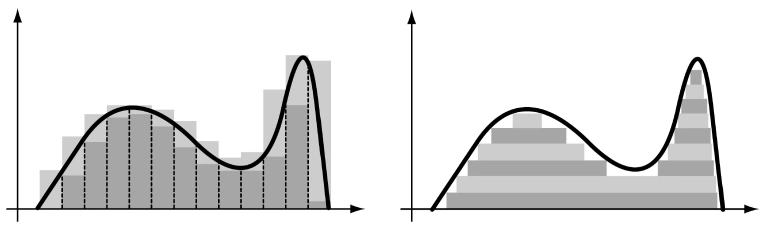
\includegraphics[width=0.75\linewidth]{img/riemann-vs-lebesgue.png}
  \vspace{0.5cm}
  \caption[Riemann and Lebesgue approximations]{Riemann and Lebesgue approximations \cite{schilling2017measures}}
  \label{figure:schilling}
\end{figure}

$$L_k^n=\{x\in\KK \,|\, t_k^n\le f(x)\le t_{k+1}^n\}.$$

Then the following approximation is usable for the area bounded by $f(D), y=0, x=a$ and $x=b$ for $D=[a,b]$, which coincides with Riemann integral.

\begin{equation}
  \label{example:lebesgue-partition}
  I_n=\sum\limits_{k=0}^{m_n-1}(t_{k+1}-t_k)\lambda(L_k^n).
\end{equation}

The additional requirement is that each $L^n_k$ is Lebesgue measurable. In Riemann integral, the function $f$ is required to be discontinuous at finite number of points, which is less general than Lebesgue measurability. Furthermore, Equation \ref{example:lebesgue-partition} can be generalized for abstract set $\Omega$ rather than $\RR^d$, its $\sigma$-algebra $\F$ and a measure $\mu$. In such measure space $(\Omega, \F, \mu)$, we will formally construct the Lebesgue integral for each measurable function $f:\Omega\to\RR$. The idea is to approximate $f$ by the limit of a sequence of steps function $(f_n)_{n\in\NN}$.

\begin{definition}[Step function]
  Let $(\Omega, \F, \mu)$ be a measure space. A function $f:\Omega\to\RR$ is a \textbf{step function}\index{step function} if there exists $\{E_n\}_{n=1}^N\subset\Omega$ and $\{c_n\}_{n=1}^N\subset\RR$ such that
  \begin{equation}
    f(x)=\sum\limits_{i=1}^nc_i\mathbf{1}_{A_i}(x).
  \end{equation}
\end{definition}

\begin{proposition}
  \label{proposition:standard-representation-of-a-step-function}
  Let $(\Omega, \F, \mu)$ be a measure space. Let $f:\Omega\to(0,\infty)$ be a positive step function. Then there exists a disjoint family $\{E_n\}_{n=1}^N\subset\Omega$ of nonempty sets, and a distinct set $\{c_n\}_{n=1}^N$ of positive number, such that
  \begin{equation}8
    f(x)=\sum\limits_{n=1}^Nc_n\mathbf{1}_{E_n}(x).
  \end{equation}
  Moreover, this representation is unique.
\end{proposition}
\begin{proof}
  If there exist non-disjoint $A_i$ and $A_j$, we rewrite
  $$c_i\mathbf{1}_{A_i}(x) + c_j\mathbf{1}_{A_j}(x) = c_i\mathbf{1}_{A_i\setminus A_j}(x) + (c_i+c_j)\mathbf{1}_{A_i \cap A_j}(x) + c_j\mathbf{1}_{A_j\setminus A_i}(x),$$
  to achieve a disjoint family.

  If there exist $c_i = c_j$, we rewrite
  $$c_i\mathbf{1}_{A_i}(x) + c_j\mathbf{1}_{A_j}(x) = (c_i+c_j)\mathbf{1}_{A_i}(x) + c_j\mathbf{1}_{A_j\setminus A_i}(x).$$

  Then the attained subset of $\RR$ is disjoint. Let us abuse the original notation
  $$f(x)=\sum\limits_{n=1}^N c_n\mathbf{1}_{E_n}(x)$$
  for this new representation. For each $E_n, n\in\{1,\ldots,N\}$, choose $x_n\in E_n$. We have $f(x_n) = c_n > 0$. Now, consider two such representations
  $$f(x)=\sum\limits_{n=1}^Nc_n\mathbf{1}_{E_n}(x) = \sum\limits_{m=1}^Md_m\mathbf{1}_{B_m}(x).$$

  If $\bigcup_{n=1}^N E_n\setminus \bigcup_{m=1}^M B_m \ne \varnothing$, taking an element $x_0$ in this difference yields a contradiction when computing $f(x_0)$. Therefore, $\bigcup_{n=1}^N E_n\setminus \bigcup_{m=1}^M B_m = \varnothing$. Similar argument shows that $\bigcup_{n=1}^N E_n = \bigcup_{m=1}^M B_m$. Hence, for each $E_n, n\in\{1,\ldots, N\}$, there exists $B_m$ where $m\in\{1,\ldots,M\}$ such that $E_n\cap B_m\ne \varnothing$. Take $x_1\in E_n\cap B_m$, we have $f(x_1) = c_n = d_m$. If $E_n\setminus B_m \ne \varnothing$, take $x_2$ in this difference, then $f(x_2) = c_n = d_k$ for some $k\in\{1,\ldots,M\}$, a contradiction to the fact that $\{d_m\}$ is disjoint. Therefore, $E_n = B_m$. Thus, the representation is unique.
\end{proof}
\begin{remark}
  The representation in Proposition \ref{proposition:standard-representation-of-a-step-function} is called the standard representation. We can check that each positive step function $f$ has the standard representation
  \begin{equation}
    f(x) = \sum\limits_{t\in f(\Omega)} t\mathbf{1}_{\{x\in \Omega : f(x) = t\}}(x).
  \end{equation}
  If $f = 0, a.e.$, we choose the representation $f(x) = 0\cdot \mathbf{1}_{\Omega}(x)$. Let us denote by $\S^+$ the set of nonnegative step functions.
\end{remark}

\begin{corollary}
  Let $(\Omega, \F, \mu)$ be a measure space. Let $f:\Omega\to\RR$ be a step function. Then there exist a unique pair $f^+, f^-\in \S^+$ such that $f = f^+ - f^-$.
\end{corollary}

\begin{definition}[Lebesgue Integral of a Step Function]
  Let $(\Omega,\F,\mu)$ be a measure space and $f(x)=\sum\limits_{i=1}^nc_i\mathbf{1}_{A_i}(x)$ be a step function. The Lebesgue integral of $f$ with respect to a measure $\mu$ is defined as
  $$\int_\Omega f \d \mu = \sum\limits_{i=1}^nc_i\mu(A_i).$$
\end{definition}

We can see that the Lebesgue integral of a step function $f$ whose value coincides with the Riemann integral of $f$.

\begin{proposition}
  \label{proposition:integral-of-almost-everywhere-equal-step-functions}
  Let $(\Omega, \F, \mu)$ be a measure space and $f\in\S^+$. Suppose that $\Omega = E\cup E^c$, where $\mu(E^c) = 0$. Define a function $\tilde{f}:\Omega\to\RR$ as
  $$\tilde{f}(x) =\begin{cases}
      f(x), & \text{ if } x\in E    \\
      a,    & \text{ if } x\in E^c.
    \end{cases}$$
  Then $\int_\Omega f \d \mu = \int_\Omega \tilde{f} \d \mu$.
\end{proposition}

\begin{proof}
  We have
  \begin{align*}
    \int_\Omega \tilde{f} \d \mu
     & = \sum\limits_{t\in \tilde{f}(\Omega)} t\mu\left(\{x\in \Omega : \tilde{f}(x) = t\}\right)                                                                                                \\
     & = \sum\limits_{t\in \tilde{f}(\Omega)} t\mu\left(\{x\in E : \tilde{f}(x) = t\}\right) + \underbrace{a\mu(E^c)}_{0}                                                                        \\
     & = \sum\limits_{t\in \tilde{f}(\Omega)} t\mu\left(\{x\in E : \tilde{f}(x) = t\}\right)                                                                                                     \\
     & = \sum\limits_{t\in \tilde{f}(\Omega)} t\mu\left(\{x\in E : \tilde{f}(x) = t\}\right) + \underbrace{\sum\limits_{t\in \tilde{f}(\Omega)} t\mu\left(\{x\in E^c : \tilde{f}(x) = t\}\right)
    }_{0}                                                                                                                                                                                        \\
     & = \sum\limits_{t\in \tilde{f}(\Omega)} t\left[\mu\left(\{x\in E : \tilde{f}(x) = t\}\right) + \mu\left(\{x\in E^c : \tilde{f}(x) = t\}\right)\right]                                      \\
     & \sum\limits_{t\in \tilde{f}(\Omega)} t\mu\left(\{x\in \Omega : \tilde{f}(x) = t\}\right)                                                                                                  \\
     & = \int_\Omega f \d \mu.
  \end{align*}
\end{proof}

\begin{definition}
  Let $f:\Omega\to[0,\infty)$ be measurable. The Lebesgue integral of $f$ is defined as
  \begin{equation}
    \int_\Omega f\d \mu = \sup\left\{\int\limits h\d \mu : h\in\S^+, h\le f\right\}.
  \end{equation}
\end{definition}

\begin{definition}
  Let $f:\Omega\to\RR$ be measurable. Define $f^+(x) = \sup(f,0)$ and $f^-(x) = \sup(-f,0)$. The Lebesgue integral of $f$ is defined as
  \begin{equation}
    \int_\Omega f\d \mu = \int_\Omega f^+\d \mu - \int(-f^-)\d \mu
  \end{equation}
  Then $f$ is said to be integrable or summable if $\int_\Omega f\d \mu<\infty$.
\end{definition}

\begin{definition}
  Let $f:\Omega\to\RR$ be measurable and $E \in \F$. The integral of $f$ over $E$ is defined as
  \begin{equation}
    \int_E f\d \mu = \int_\Omega f\mathbf{1}_E\d \mu.
  \end{equation}
\end{definition}

\begin{remark}
  When $(\Omega, \F, \mu) = (\RR^d, \B{(\RR^d)}, \lambda)$, Lebesgue integral coincides with Riemann integral. In such case, we simply write
  \begin{equation}
    \int_B f\d\lambda = \int_B f(x)\d x, B\in\B(\RR^d).
  \end{equation}
\end{remark}

\begin{proposition}
  \label{proposition:integral-of-le-everywhere-functions}
  Let $(\Omega,\F,\mu)$ be a measure space. Let $f$ and $g$ be measurable functions such that $f\le g, \mu-a.e.$ Then
  \begin{equation}
    \int_\Omega f\d \mu \le  \int_\Omega g\d \mu.
  \end{equation}
\end{proposition}

\begin{proof}
  If $f\le 0  \le g, \mu-a.e.$, we can use step functions approximation to prove that $\int_\Omega f\d \mu \le 0 \le  \int_\Omega g\d \mu$. If $f\le g\le 0$, we will prove that $0\le \int_\Omega -g\d \mu \le \int_\Omega -f\d \mu$. Hence, let us consider the case $ 0  \le f\le  g, \mu-a.e.$ Denote $E = \{x\in \Omega : f(x) \le g(x)\}$, we have $\mu(E^c) = 0$. For a step function $h\in S^+$, define $\tilde{h}$ similarly as in Proposition  \ref{proposition:integral-of-almost-everywhere-equal-step-functions}. We have
  \begin{align*}
    \int_\Omega f\d \mu
     & = \sup\left\{\int_\Omega f\d \mu : h\in \S^+, h\le f\right\}                                  \\
     & = \sup\left\{\int_\Omega f\d \mu : \tilde{h}\in \S^+, \tilde{h}\le f \text{ on } E\right\}    \\
     & \le  \sup\left\{\int_\Omega f\d \mu : \tilde{h}\in \S^+, \tilde{h}\le g \text{ on } E\right\} \\
     & =  \sup\left\{\int_\Omega f\d \mu : \tilde{h}\in \S^+, h\le g\right\}                         \\
     & =  \int_\Omega g\d \mu.
  \end{align*}
\end{proof}

\begin{corollary}
  \begin{enumerate}[label=(\roman*), ref=(\roman*)]
    \item []
    \item If $f = g, \mu-a.e.$, then $\int_\Omega f\d \mu =  \int_\Omega g\d \mu$.
    \item If $\int_\Omega |f|\d \mu = 0$, then $f=0,\mu-a.e.$
  \end{enumerate}
\end{corollary}

\begin{proof}
  For statement (i), we have $f\le g$ and $g\le f$, $\mu$-a.e. The conclusion follows directly from Proposition \ref{proposition:integral-of-le-everywhere-functions}. For statement (ii), let $E = \{x\in\Omega : |f(x)| = 0\}$, we have
  \begin{align*}
    0
     & = \int_\Omega |f|\d \mu                    \\
     & = \int_E |f|\d \mu + \int_{E^c} |f|\d \mu  \\
     & = \int_{E^c} |f|\d \mu                     \\
     & \ge \int_{E^c} \inf\limits_{E^c} |f|\d \mu \\
     & = \inf\limits_{E^c} |f| \mu (E^c)          \\
     & \ge 0
  \end{align*}
  Thus, $\mu (E^c)=0$ or $f=0$, $\mu$-a.e.
\end{proof}

To conclude this discussion of Lebesgue integral, we introduce $L^p$ spaces, crucial Banach spaces in functional analysis, particularly relevant for theorems in stochastic processes.

\begin{definition}
  \label{definition:Lp-space}
  Let $(\Omega,\F,\mu)$ be a measure space and $p\ge1$. The $L^p := L^p(\mu)$ space includes every function $f:\Omega\to\RR^m$, such that
  $$\left(\int\limits_\Omega \|f\|^p_p\d \mu\right)^{1/p}<\infty.$$
\end{definition}

\begin{remark}
  We can also define $L^\infty$ space. However, in the scope of the project, let us focus on $L^2$ onward. Those keen on delving deeper can refer to popular textbooks on Measure Theory \cite{cohn2013measure} or Functional Analysis \cite{rudin1987functional}.
\end{remark}

\begin{theorem}
  \label{theorem:L2-is-Banach}
  The $L^2$ space in Definition \ref{definition:Lp-space} is a vector space. The function $\|\cdot\|_{L^2} : L^2\to\RR$ be defined by
  $$\|f\|_{L^2(\mu)}=\left(\int\limits_\Omega f^2(x)\d \mu\right)^{1/2}, \forall f\in L^2.$$
  is a norm in the $L^2$ space. Moreover, the normed space $(L^2, \|\cdot\|_{L^2})$ is Banach.
\end{theorem}

\begin{proof}
  Firstly, we prove that $L^2$ is a vector space. Let $f,g \in L^2$, it is sufficient to show that $f+kg\in L^2$, for $k\in\RR$. Indeed, we have
  \begin{align*}
    \left(\int\limits_\Omega \|f + kg\|^2_2\d \mu\right)^{1/2}
     & \le \left(\int\limits_\Omega \left(\|f\|^2_2 + k^2\|g\|^2_2\right)\d \mu\right)^{1/2}                               \\
     & = \left(\int\limits_\Omega \|f\|^2_2\d \mu\right)^{1/2}  + \left(k^2\int\limits_\Omega \|g\|^2_2\d \mu\right)^{1/2} \\
     & < \infty.
  \end{align*}
  Now we prove that $\|\cdot\|_{L^2}$ is a norm. Nonnegativity and homogeneity are straightforward. Note that the function
  $\langle \cdot, \cdot\rangle : L^2 \times L^2\to \RR$ defined by
  \begin{equation}
    \langle f,g \rangle = \int\limits_\Omega fg \d \mu, \forall f,g\in L^2
  \end{equation}
  is a dot product in $L^2$. Using Cauchy-Schwarz inequality for any $f,g\in L^2$, we have
  \begin{align*}
    \|f + g\|_{L^2}^2
     & = \int\limits_\Omega \|f + g\|^2_2\d \mu                                                                                                                             \\
     & = \int\limits_\Omega (\|f\|_2 +\|g\|_2)^2\d \mu                                                                                                                      \\
     & = \int\limits_\Omega \|f\|_2^2\d \mu + \int\limits_\Omega \|g\|_2^2\d \mu + 2\int\limits_\Omega \|f\|_2\|g\|_2\d \mu                                                 \\
     & \le  \int\limits_\Omega \|f\|_2^2\d \mu + \int\limits_\Omega \|g\|_2^2\d \mu + 2\left(\int\limits_\Omega \|f\|_2\d \mu \int\limits_\Omega \|g\|_2\d \mu\right)^{1/2} \\
     & = \left( \left(\int\limits_\Omega \|f\|_2\d \mu\right)^{1/2} + \left(\int\limits_\Omega \|g\|_2\d \mu\right)^{1/2} \right)^2                                         \\
     & = \left(\|f\|_{L^2} + \|g\|_{L^2}\right)^2.
  \end{align*}
  Thus, triangle inequality is also satisfied.

  Finally, we prove that $L^2$ is complete. Consider a sequence $(f_n)_{n=1}^\infty\subset L^2$ such that $\lim\limits_{n\to\infty}\|f-f_n\|_{L^2}$. We have $\|f\|_{L^2}\le \|f-f_n\|_{L^2} + \|f_n\|_{L^2}, \forall n\in \NN$. Therefore,
  $$\|f\|_{L^2} \le \lim\limits_{n\to\infty}\left(\|f-f_n\|_{L^2} + \|f_n\|_{L^2}\right) = \lim\limits_{n\to\infty} \|f_n\|_{L^2} < \infty.$$
\end{proof}

Moreover, we can easily prove that the function $\langle\cdot,\cdot\rangle : L^2\times L^2\to\RR_+$ defined by
\begin{equation}
  \langle f,g\rangle = \int\limits_\Omega fg \d \mu
\end{equation}

is an inner product.
